\chapter{Object detection}
Object detection is another prevalent task in the domain of computer vision.
An object detection task is one where the goal is to localize one or many different classes of objects using bounding boxes.
Before current deep learning-based techniques, a popular way to solve the problem was to use handcrafted features like in image classification and to use a sliding window over the image for localizing objects.
These previous techniques include, for example, the Viola-Jones detector \citep{viola-jones}, which uses a sliding window and AdaBoost for features, and another popular method was using histograms of oriented gradients \citep{hogs} to find where the boundaries of objects exist.
These days there exist various ways of using the feature maps of neural networks for learning the filters to get much better results.
The various architectures can be split into two approaches, one-stage detectors, and two-stage detectors.
The two-stage detectors require region proposals, based on which the object detection is done.
An often-used family of these kinds of methods is the R-CNN classifiers, for example, the faster R-CNN \citep{faster-rcnn}.
In the one-stage detectors, features from various layers of the classifier are used to get the predictions.
For example, the YOLOv4 \citep{yolov4} is the 4th iteration of the single-stage YOLO family of detectors that are very popular due to the good balance between fast speed and good accuracy.

\section{Metrics}
The training of object detection models requires data sets that have been labeled for that purpose.
Generally, the data sets contain bounding box annotations for each of the classes in the data set, such as seen in Figure 5.1.
For this reason, object detection models can't use a simple metric like the basic accuracy in image classification.
As the images are often manually labeled, the boxes are most likely not completely consistent.
So most likely, the predictions are never going to align with the labeled boxes perfectly.
Consequently, the method for evaluating object detection performance is Average Precision (AP) or mean Average Precision (mAP) or one of their variants.
These metrics use intersection over union (IoU) score to evaluate how incorrect the predicted bounding box is when compared to the actual label. Intersection over union is visualized in Figure 5.1.

\begin{figure}[h!]
    \centering
    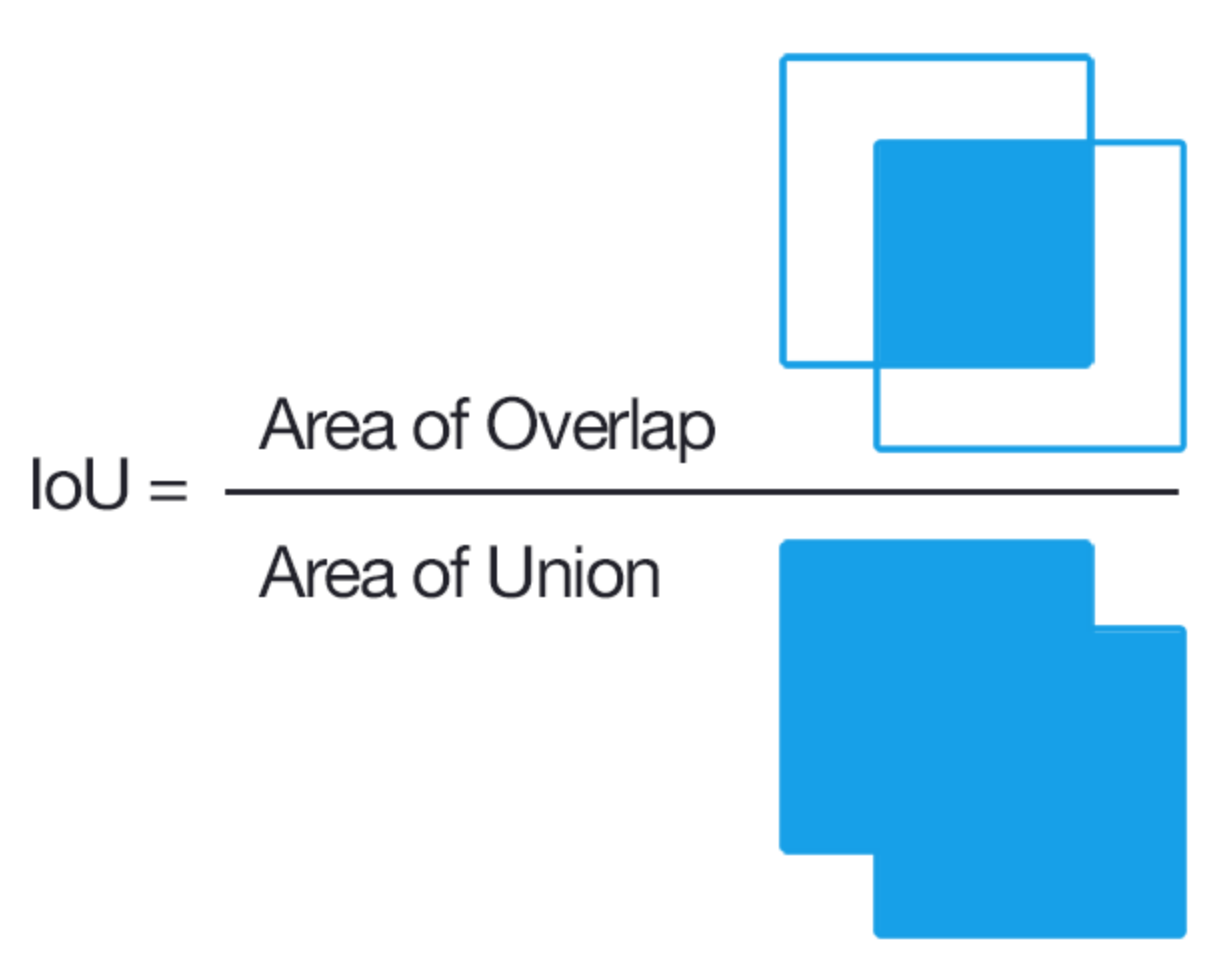
\includegraphics[width=0.8\textwidth]{imgs/intersection_over_union.png}
    \caption{The visual formula for calculating intersection over union.}
\end{figure}

To get to a final AP score, the first thing that has to be decided is the IoU score threshold for considering a prediction to be correct.
For example, we could consider all predictions that have over 50\% or 75\% overlap in the IoU.
The threshold value for IoU that should be used is not entirely standardized, and there are multiple ways of calculating the AP score.
For example, the popular COCO dataset \citep{COCO} uses an average of 10 IoU scores ranging from .5 to .95 IoU thresholds as the main metric.
To get the AP for a class, we need to graph the precision-recall curve and then calculate the area under it.
For example, the Pascal Visual Object Classes Challenge (VOC) \citep{PVOC} recommends doing this by using 11 points of interpolated precision.
So we get the following formula for Average Precision:

\[AP = \frac{1} {11} \sum_{r \in \{0, 0.1, \ldots, 0.9 , 1\}}{p_{interp}(r)}\] \noindent

Where $p_{interp}$ is defined as

\[p_{interp}(r) = \max \limits_{\tilde{r}:\tilde{r} \geq r} p(\tilde{r})\]

Then to get the mAP score, we can average the AP score for each of the classes in the data set.
As was mentioned, this way of calculating the AP is not always the same, for example, the COCO metrics \citep{COCO_SITE} recommend using 101 points for integrating the curve instead of the 11 proposed in the VOC.
This discrepancy in the integration means that not all AP scores are directly comparable.

\section{Object detection model structure}
Much like image classifiers and many other vision tasks, modern object detectors rely on pre-trained backbones to generate the features required for predicting bounding boxes.
A classifier head is required to get these predictions, but in object detectors, this head is more complicated than in image classification.

For the backbone, most object detection architectures use one of the same ImageNet models as in image classification such as ResNet or VGG.
However, the YOLO models use DarkNet, which is specifically designed for achieving efficient results in object detection \citep{yolov4}.
The main reason for picking one backbone over another is often a function of both accuracy and inference time.
As object detectors are often run on video data, inference time can be more significant than in image classification, as it is often desirable to be able to run them in real-time.

The head is where the architectures differ the most, and generally, any backbone could be combined with a specific detector head.
The head comprises of a neck, which connects the intermediate features from the backbone to the final head.
The intermediate features are generally connections from some specific layers of the backbone.
Earlier single-stage detectors used the extracted features directly, but the current state-of-the-art methods use special feature pyramids and path aggregation to get the best results \citep{efficientDet}
For example, the YOLO v4 uses spatial pyramid pooling \citep{SPP} over the DarkNet features and path aggregation net \citep{PANET} to concatenate the parameters for the classifier head \citep{yolov4}.

In two-stage detectors like faster R-CNN \citep{faster-rcnn}, there is a region proposal network (RPN), which predicts region proposals using a sliding window for some anchor boxes.
Running this RPN is expensive, and often the two-stage models are much slower than the single-stage detectors.
The benefit of the two-stage approach is generally a better accuracy. 
Still, recently the one-stage methods like YOLO v4 have achieved very similar accuracies to the two-stage ones with much faster inference times \citep{yolov4}.

\section{Multi-dataset training}
Often an object detection problem requires detecting multiple different classes in a similar context.
For example, a self-driving car would need to detect various traffic signs, cars, pedestrians, road markings, cyclists, and many other things.
Collecting a single dataset that has labels for all of the classes of interest can be a very daunting task.
Even if it is feasible to create the dataset for the original classes of interest, this approach does not scale very well when new classes need to be recognized.
As likely the original dataset might contain millions of images labeled for multiple classes, adding a new class would require going through the entire dataset again and labeling the new class as well.
The new class may be relatively rare; for example, we may be interested in detecting emergency vehicles with sirens on.
Here is where multi-dataset learning is highly beneficial as it only allows for collecting a specific class dataset.
This type of cross-dataset learning is useful when we need to combine multiple distinct data sources to detect some union of the labels \citep{cross_data}.

The main difficulty in combining multiple datasets for detection lies in the fact that they likely contain unlabeled overlapping classes.
For example, given a dataset for detecting cars and another for detecting stop signs, we have two distinct datasets where only one of the classes is labeled.
If we train this model, assuming that the labels are genuinely valid, we will end up unlearning the tasks due to the overlap of the classes.
The problem lies in the fact that it is most likely that in the car dataset, we will find stop signs that are not labeled.
Similarily we will find cars that are unlabeled within the stop sign dataset.
When we naively train this model, we will end up detecting cars and stop signs that are actually correct but incorrect based on the labels.
The model will be punished for detecting these non-labeled positive examples due to the absence of the labels.

One way to do this is by disallowing the labels from incorrect datasets affecting the total loss.
For example, in \citep{cross_data}, the RetinaNet \citep{retinaNet} model's loss function is modified to ignore the losses for tasks that are not a part of the dataset.
This way, each class will get its own positive and negative dataset to train on and not affect the performance of the other classes.
Still, this does not completely solve the problem as some of the classes might require conflicting features, as can be the case when very different tasks are combined. 
In that case, it could be smart to split the similar classes into different detectors and maybe share only the lower levels between all tasks.

Similar multi-dataset training can also be applied in multi-label image classification settings.
A multi-label image classification problem is one where we want to assign multiple labels to an image.
For example, we might want to classify whether it is raining, the sun is shining, the sea is visible, is there a dog in the image, and so on for all the classes of interest.
Again, collecting a dataset containing all labels for all images is quite expensive, but we can train this with a separate binary classification head for each task.
And as collecting a separate dataset for each task is relatively easy, it is possible to create a quite powerful model with relative ease.

\section{Self-supervised object detection}


\section{EfficientDet}